\section{Methods}
\label{sec:methods}

\begin{figure*}
\center
\resizebox{5in}{!}{
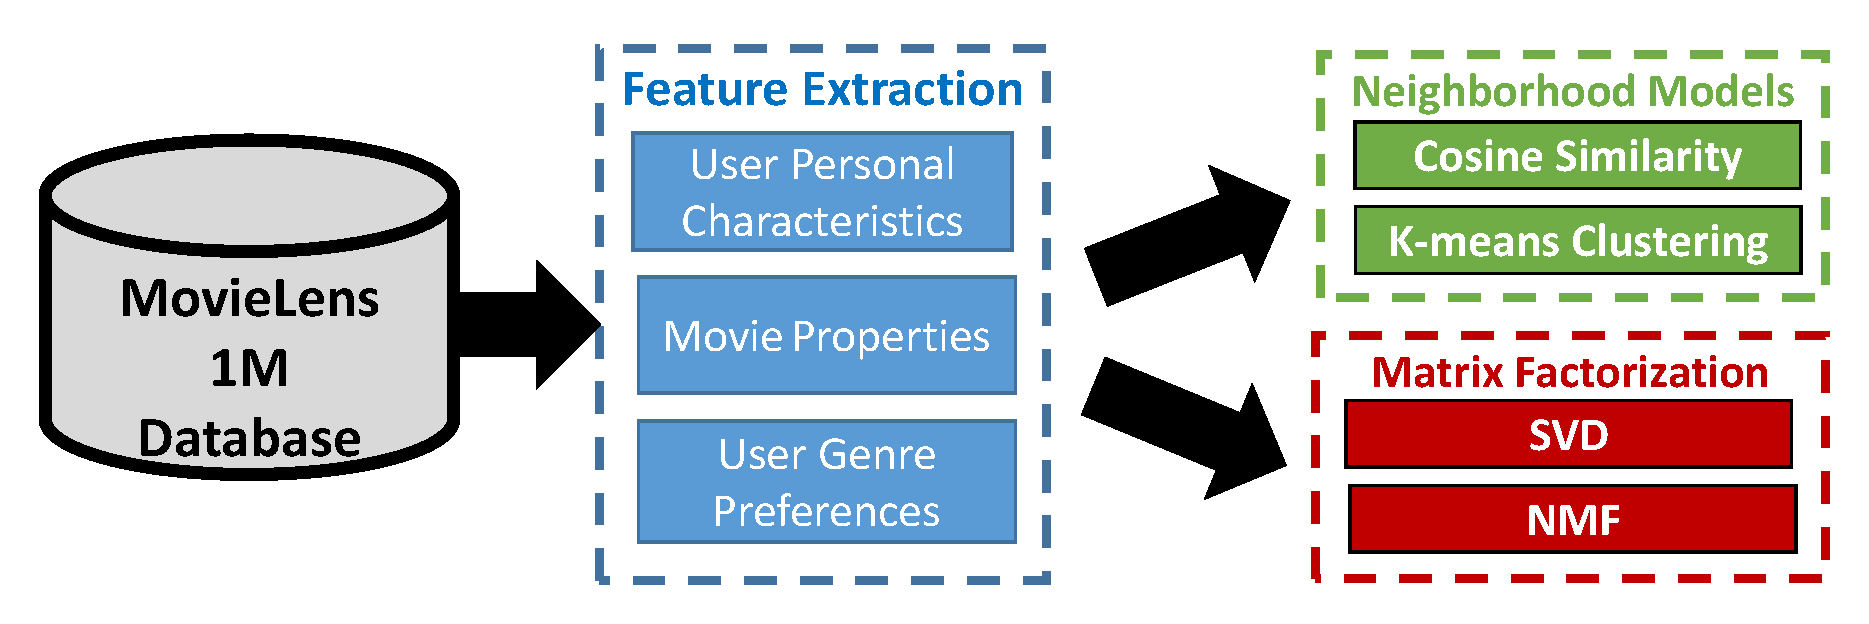
\includegraphics{figures/methods_pipeline.pdf} 
}
\caption{The movie recommendation prediction flow}
\label{fig:methods_pipeline}  
\end{figure*}


We now go over the various techniques we employed for the movie dataset analysis and for the purpose of predicting recommended movies.
Figure~\ref{fig:methods_pipeline} outlines the general prediction flow and techniques we used in our work.


\subsection{Feature Extraction}

\begin{table}
\begin{center}
\resizebox{5.7in}{!}{
\begin{tabular}{|c|l|l|l|l|l|l|l|l|l|l|l|l|l|l|l|l|l|l|l|l|l|l|l|l|l|l|}
\hline
%\textbf{userId} & \textbf{gender} & \textbf{age} & \textbf{occupation} & \textbf{Mystery} & \textbf{Sci-Fi} & \textbf{Crime} & \textbf{Drama} & \textbf{Animation} & \textbf{IMAX} & \textbf{Action} & \textbf{Comedy} & \textbf{Documentary} & \textbf{War} & \textbf{Romance} & \textbf{Horror} & \textbf{Film-Noir} & \textbf{Musical} & \textbf{Fantasy} & \textbf{Adventure} & \textbf{Children} & \textbf{Thriller} & \textbf{Western} & \textbf{rate\_num} & \textbf{rate\_avg} & \textbf{rate\_std} & \textbf{avg\_score\_diff} \\
\textbf{userId} & \textbf{G} & \textbf{A} & \textbf{O} & \textbf{My} & \textbf{SF} & \textbf{Cr} & \textbf{Dr} & \textbf{An} & \textbf{I} & \textbf{Ac} & \textbf{Co} & \textbf{Do} & \textbf{W} & \textbf{Ro} & \textbf{Ho} & \textbf{FN} & \textbf{Mul} & \textbf{Fa} & \textbf{Ad} & \textbf{Ch} & \textbf{Th} & \textbf{We} & \textbf{rate\_num} & \textbf{rate\_avg} & \textbf{rate\_std} & \textbf{avg\_score\_diff} \\
\hline
457 & M & 18 & 4 & 38 & 121 & 105 & 409 & 8 & 0 & 199 & 254 & 10 & 100 & 90 & 76 & 13 & 7 & 27 & 73 & 5 & 196 & 4 & 237 & 3.71308 & 0.905887 & -0.021912\\
\hline
2768 & M & 25 & 17 & 14 & 46 & 38 & 140 & 13 & 0 & 79 & 88 & 3 & 37 & 27 & 8 & 12 & 8 & 9 & 18 & 12 & 74 & 8 & 80 & 4.0375 & 0.797555 & 0.108199\\
\hline
1980 & M & 35 & 7 & 170 & 351 & 275 & 1977 & 130 & 0 & 631 & 1733 & 45 & 206 & 797 & 253 & 60 & 177 & 122 & 388 & 288 & 590 & 65 & 1260 & 3.48254 & 1.026094 & 0.019891\\
\hline
402 & M & 25 & 11 & 8 & 61 & 178 & 372 & 9 & 0 & 140 & 734 & 0 & 53 & 187 & 34 & 8 & 9 & 27 & 76 & 21 & 96 & 19 & 284 & 3.591549 & 0.873353 & 0.023182\\
\hline
4126 & M & 25 & 17 & 32 & 224 & 80 & 300 & 122 & 0 & 456 & 416 & 0 & 69 & 224 & 112 & 4 & 63 & 91 & 253 & 191 & 282 & 37 & 358 & 3.513966 & 0.902248 & 0.08732\\
\hline
3418 & F & 18 & 3 & 38 & 64 & 66 & 322 & 51 & 0 & 86 & 313 & 10 & 67 & 172 & 14 & 20 & 90 & 9 & 28 & 92 & 121 & 12 & 211 & 3.791469 & 1.221499 & 0.130147\\
\hline
112 & M & 18 & 6 & 87 & 291 & 139 & 817 & 265 & 0 & 571 & 642 & 11 & 117 & 315 & 231 & 32 & 148 & 83 & 311 & 308 & 481 & 23 & 679 & 3.441826 & 1.240844 & 0.0129\\
\hline
3119 & M & 45 & 1 & 4 & 166 & 6 & 46 & 4 & 0 & 191 & 70 & 0 & 36 & 15 & 11 & 3 & 5 & 50 & 126 & 35 & 64 & 15 & 90 & 3.377778 & 1.269976 & -0.259006\\
\hline
1737 & M & 35 & 20 & 93 & 465 & 173 & 585 & 85 & 0 & 884 & 967 & 3 & 127 & 341 & 363 & 15 & 48 & 82 & 413 & 154 & 666 & 26 & 775 & 3.410323 & 0.984733 & 0.329893\\
\hline
1322 & M & 56 & 0 & 111 & 130 & 81 & 587 & 86 & 0 & 192 & 743 & 5 & 132 & 274 & 16 & 35 & 260 & 49 & 236 & 143 & 88 & 89 & 384 & 4.117188 & 0.803194 & 0.3565\\
\hline
\end{tabular}
}
\end{center}
\caption{Representative Users and Features (G=Gender, A=Age, O=Occupation, My=Mystery, SF=Sci-Fi, Cr=Crime, Dr=Drama, An=Animation, I=IMAX, Ac=Action, Co=Comedy, Do=Documentary, W=War, R=Romance, H=Horror, FN=Film-Noir, Mu=Musical, Fa=Fantasy, Ad=Adventure, Ch=Children, Th=Thriller, We=Western)}

\label{tab:rep_users}
\end{table}





In order to analyze the MovieLens dataset, we first extracted several features, for the movies and users separately. 

\textbf{Basic Movie Features} 
\begin{itemize}
\item Binary genres vector representing all the genres included in the movie. Each movie follows the genre standard of IMDB (Internet Movie Database, www.imdb.com). Each movie is categorized to a minimum of one genre, and a maximum of five.
\item Average rating by all users
\item Overall number of ratings
\item Ratings standard deviation
\end{itemize}

\textbf{Basic User Features} 
\begin{itemize}
\item Age
\item Gender
\item Number of ratings
\item Occupation
\item Average rating given by the user
\item Overall number of ratings
\item Ratings standard deviation
\end{itemize}

After the basic feature extraction, we further analyzed the existing features to create additional user features:

\textbf{User Genres Preference}

To represent the user genre prefrence based on past ratings, we created a score that captures the average rating of a user for each genre: 
\begin{equation} score\_for\_movie\_genre(G_j) = \frac{\sum^5_{i=1}{i\times number\_of\_i\_movie\_ratings}}{Total\_number\_of\_ratings} 
\end{equation}
We created a vector of genres prefrences for each user as additional features.

\textbf{User specific effect}

As suggested by the winners of the \textit{Netflix Prize} in their paper~\cite{bell2007bellkor}, we created a feature that represent the user tendency to rate below or above the expected rating. We calculated the average difference of the user ratings from each movie average rating by all the users.

\subsection{Selecting representative test sets}
The recommendation system is based on the scenario of a specific target user. The system will predict movies ratings for this user, and therefore the test dataset is built from the users perpective. We have decided to use our set of extracted features to choose users that will properly span the feature space, and thus be better representatives than complete random selection. 

Using the abovemention set of features, we used the K-means algorithm implemented in the SciKitLearn Python libraries~\cite{pedregosa2011scikit}. By setting K=10, the users were split into k groups, from which we randomly chose 10 users, one from each group. These users will remain constant throughout our analysis, and we will try to predict the ratings for each user individually. This number of ratings is sufficient to statistically asses our methods, together with beeing computationally feasible. The representative users and their corresponding features are shown here in Table~\ref{tab:rep_users}.


\subsection{Clustering}


One of the standard approaches to collaborative filtering is to use neighborhood models. We used user-user approach which intend to find a set of similar users and base the prediction on their recorded ratings. To cluster users we used the K-means algorithm implemented in the SciKitLearn Python libraries~\cite{pedregosa2011scikit}. To determine K for the algorithm we chose to rely on a rule of thumb described in the work of Kodinariya and Makwana~\cite{kodinariya2013review}: $K\approx\sqrt{\frac{n}{2}}$. For $n=6,040$, K is approximately 50, so this is the number of clusters we used.

The prediction using clustering was created for each of the representative users individually. Using 10-fold cross-validation, we randomly chose to remove 10\% of the user ratings, and use all the rest of the dataset as training set, including all the other users and 90\% of the user ratings. We constructed the K-means clustering from the training set. Then, for each movie in the test set, we predicted the rating as the average of ratings for this movie by other users from the same cluster, and added the \textit{user specific effect} that was mentioned earlier as one of the users features. If none of the users in the cluster had rated the movie, then the rating was based on the average of all the users in the training set instead. The predicted ratings are then beeing used to rank the list of movies in the test set.

\subsection{Cosine Similarity}


\begin{figure}
\begin{tabular}{ l l l}
  \hspace{2.0cm}(a) & \hspace{4.2cm}(b) & \hspace{4.2cm}(c) \\
\end{tabular}\\
\resizebox{6in}{!}{
  \begin{tabular}{ c c c}
  \hspace{-2.8cm}
  
\includegraphics[trim={3cm 0 0 0},clip]{figures/ndcg_ratings_num.pdf} 
  &  
  \hspace{-2.5cm}
  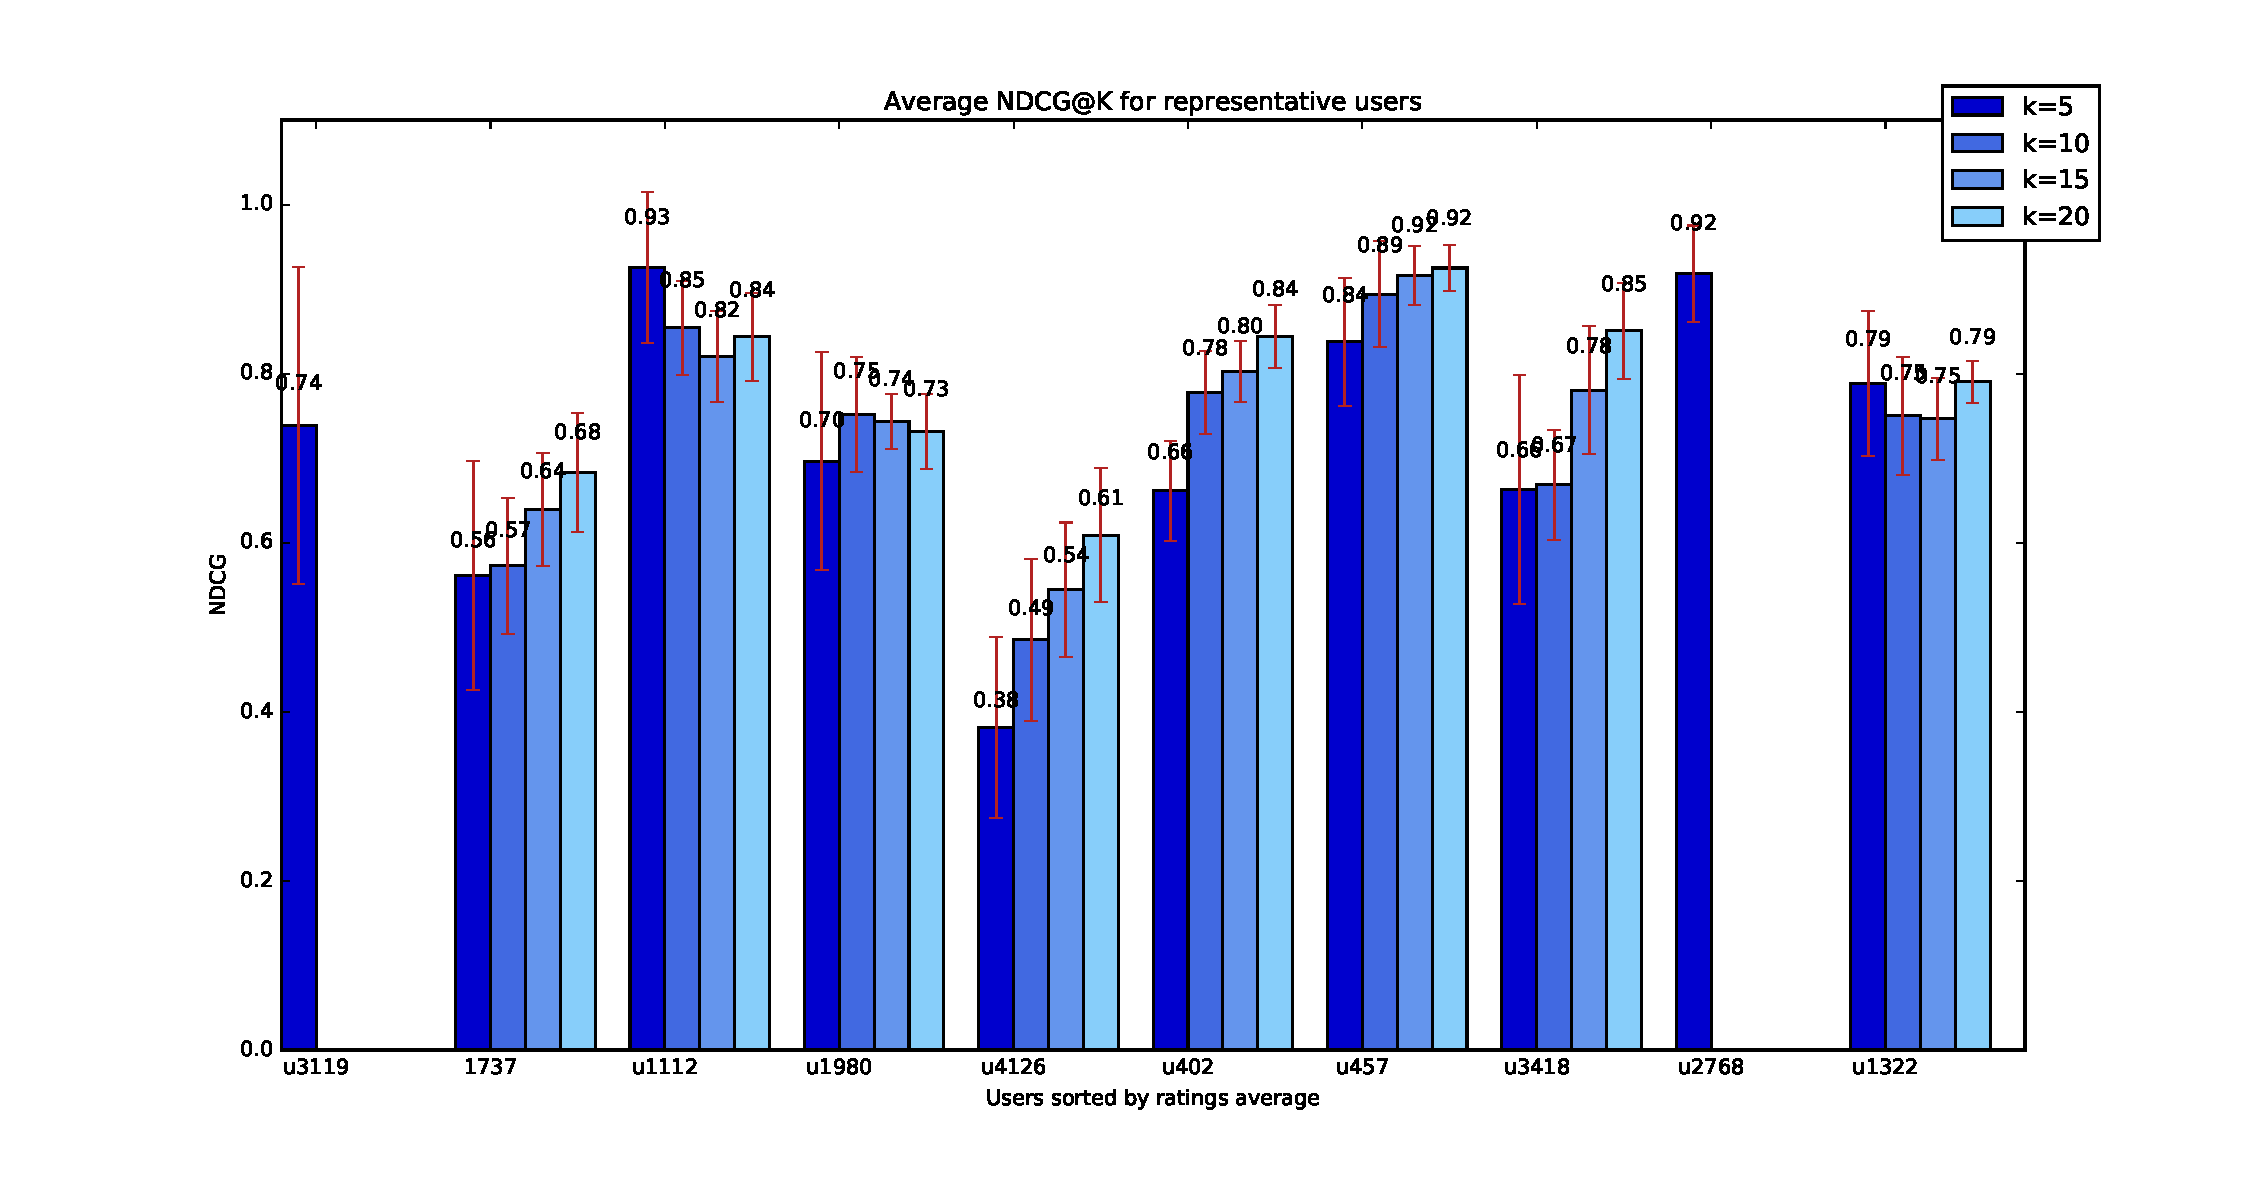
\includegraphics[trim={3cm 0 0 0},clip]{figures/ndcg_ratings_avg.pdf} 
  &
  \hspace{-2.5cm}
  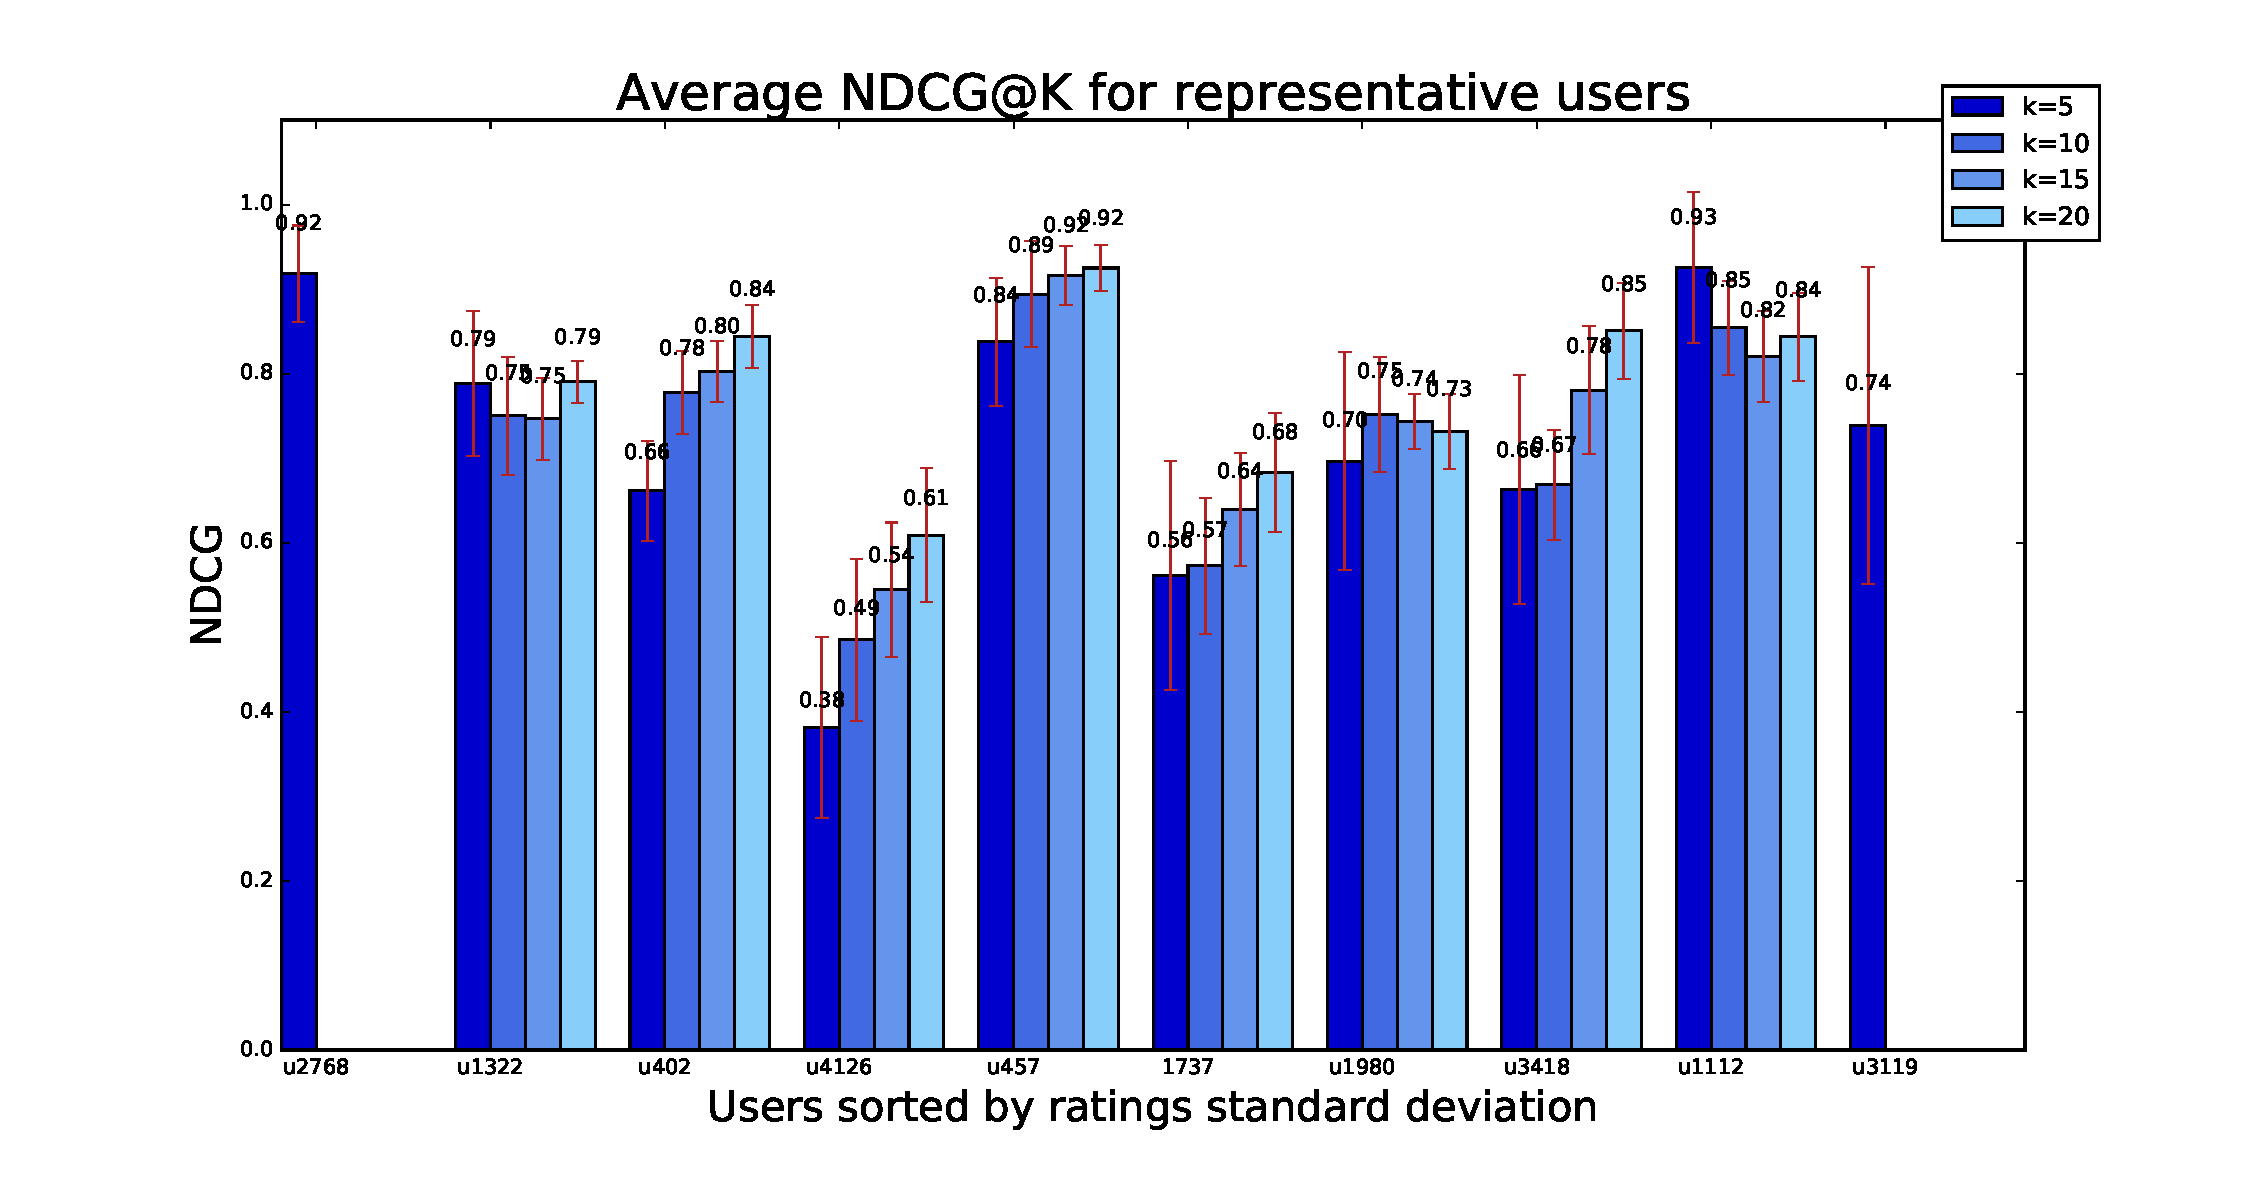
\includegraphics[trim={3cm 0 0 0},clip]{figures/ndcg_ratings_std.pdf} \\
\end{tabular}
}
\caption{Ranking movies using K-means clustering: 
\\The average NDCG@k for k=\{5, 10, 15, 20\} is shown in the bars, and the corresponding standard deviation is shown as error bars. (a) representative users sorted by number of ratings, (b) representative users sorted by average rating, (c) representative users sorted by rating standard deviation. }
\label{fig:ndcg}  
\end{figure}


A second metric we used to find a set of similar users for ratings prediction, is the cosine similarity metric, since it is a convenient technique to correlate vectors based on the relation between their members.
Feature-wise cosine similarity was calculated in the following manner. Given a feature vectors of two users $x$, and $y$: $v^x_{F}=\{\theta^x_{1},\theta^x_{2},...,\theta^x_{N}\}$,$v^y_{F}=\{\theta^y_{1},\theta^y_{2},...,\theta^y_{N}\}$
We define the cosine similarity in the following way
\begin{equation}
\footnotesize
\text{cosine\_similarity}_{x,y} = \frac{<v^x_{F},v^y_{F}>}{\sqrt{<v^x_{F},v^x_{F}}> \cdot \sqrt{<v^y_{F},v^y_{F}}>}=\frac{\sum^N_{i=1}{\theta^x_i \cdot \theta^y_i}}{{\sqrt{\sum^N_{i=1}{(\theta^x_i)^2} }}\sqrt{\sum^N_{i=1}{(\theta^y_i)^2 }}}
\label{eq:cosinesimilarity}
\end{equation}

We did the same 10-folds cross-validation we used for the k-means clustring, for the 10 representative users, with the same distribution to train and test sets in each iteration. For each of the inspected users, we rank all the users according to the cosine similarity rate defined in Equation~\ref{eq:cosinesimilarity}, based on the extracted features of the training set.
We predict the user rating for a certain movie based on the average movie rating of the N most similar users, who have rated the movie.

\begin{figure}
\center
\resizebox{4in}{!}{
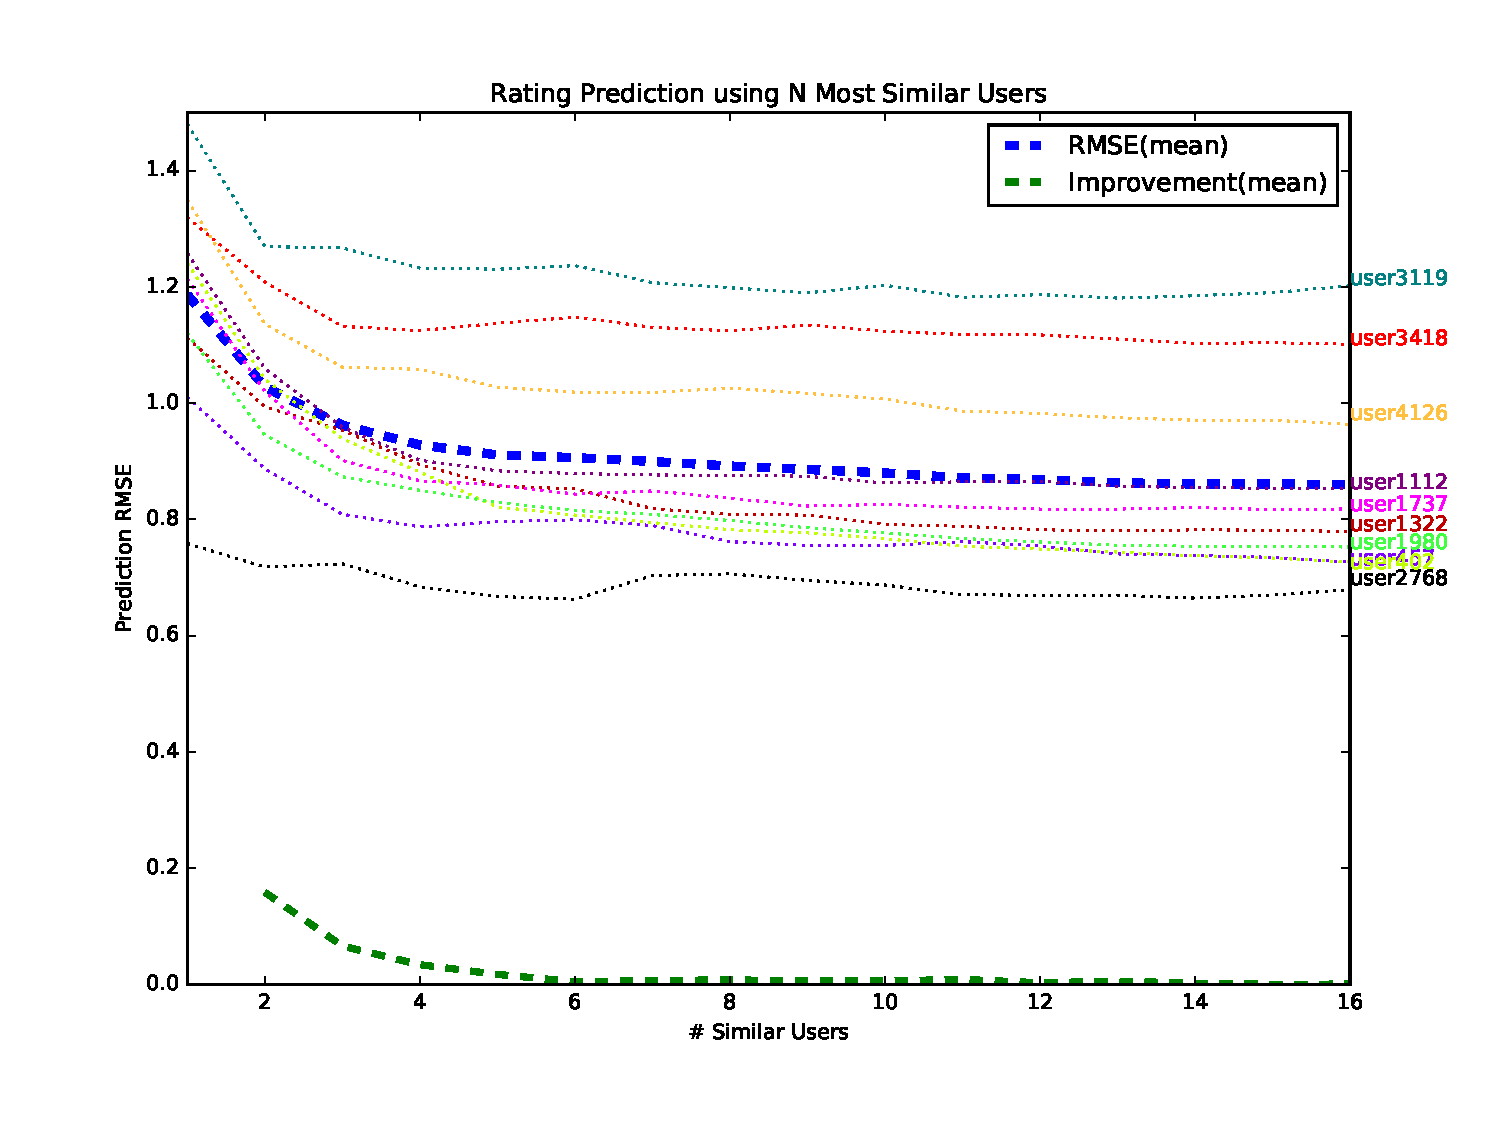
\includegraphics{figures/user_similarity.pdf} 
}
\caption{User Similarity Rating Prediction Results (RMSE vs. \# similar users)}
\label{fig:user_similarity}  
\end{figure}


\subsection{Matrix Factorization}

Matrix Factorization methods can be useful in making predictions about the topology of the underlying graph of datasets, that can be represented as sparse matrices.
We describe the user rankings database as a sparse matrix of users and movies, the sparsity of the matrix formed by ratings is: $1000209/(3,900 \cdot 6,040)\approx0.04$
We used the SVD and NMF algorithms, as implemented in the SciKitLearn Python libraries~\cite{pedregosa2011scikit}.

We performed a 10-fold cross-validation to asses our predictions, and calculate the average of the accumulated measurments from the 10 runs. 
In our first attempt, we tried to predict the actual ratings all the ratings in the training set. However, these methods produced high error rates, compared to the user similarity techniques, since they do not use the user and movie extracted features.
Therefore, we changed our prediction target to the following binary question: "will the user like this movie?"
And we reconstructed the ratings matrix as a binary matrix in which a Member[i,j] is set if the rating of user $i$ for movie $j$ is $\geq$ 4. As part of our literature survey, we encountered the work by Koren et al.~\cite{koren2009matrix}, in which they addressed the problem in a similar fashion of binarizing the ratings of movies to 4 and above. In order to choose the number of components, for each training set we preformed cross-validation within, and treated the components number as a hyperparameter. We chose the number of components that minimized the RMSE in our grid search.

